\documentclass{beamer} % change to article if necessary 
\usepackage[brazilian]{babel}
\usepackage{graphicx, txfonts} % Required for inserting images
\usepackage{amsfonts}
\usepackage{amsmath}
\usepackage{amssymb}
\usepackage{amsthm}
\usepackage{mathtools}
\usepackage{lmodern}
\usepackage{tikz}
\usepackage{cancel}
\newcommand\myalign[1]{\centerline{$\displaystyle#1$}}
\usepackage{tcolorbox} \tcbuselibrary{theorems}
\newcommand{\heart}
{\ensuremath\heartsuit}
\newcommand{\mdc}{\mathrm{mdc}}
\DeclareMathOperator{\diam}{diam}
\DeclareMathOperator{\rot}{rot}
\DeclareMathOperator{\gr}{Gr}
\DeclareMathOperator{\tr}{tr}
\newcommand{\filledheart}{\ensuremath\varheartsuit}

\usetheme{Madrid}
\usecolortheme{default}

\title[Computando a criminalidade em Manhattan]{Sobre diferentes métodos de resolução de sistemas lineares para computar os índices de criminalidade sobre um grafo de Manhattan}
\author[Vinícius, Natália, Larissa, Fábio]{Vinícius Girão \and Natália Carvalho \and Larissa Rocha \and Fábio Kauê}
\institute[ICMC]{Instituto de Ciências Matématicas e de Computação da Universidade de São Paulo}

\pdfsuppresswarningpagegroup=1

%\newtheorem{theorem}{Teorema}[section]
%\newtheorem{prop}{Proposição}[theorem]
\newtheorem{exer}{Exercício}[section]
\newtheorem{prop}{Proposição}[section]
\newtheorem{cor}{Corolário}[prop]
\newtheorem{exemplo}{Exemplo}[section]
\newtheorem{resultado}{Resultado}[section]
\newtcbtheorem[number within=section]{theorem}{Teorema}%
{colback=red!5,colframe=red!35!black,fonttitle=\bfseries}{th}
\newtcbtheorem[number within=section]{definition}{Definição}%
{colback=blue!5,colframe=blue!35!black,fonttitle=\bfseries}{df}
\newtcbtheorem[number within=section]{propp}{Proposição}%
{colback=green!5,colframe=green!35!black,fonttitle=\bfseries}{pr}
\newtcbtheorem[number within=section]{lema}{Lema}%
{colback=yellow!5,colframe=yellow!35!black,fonttitle=\bfseries}{lm}

\theoremstyle{definition}
\newenvironment{dem}{\paragraph{\textit{Dem.:}}}{\hfill$\square$}

\begin{document}
    \frame{\titlepage}

    \begin{frame}{Para os métodos iterativos...}
        \pause
        \begin{columns}
            \begin{column}{0.5\textwidth}
                \begin{enumerate}
                    \item Utilizamos uma tolerância de 1e-6.
                    \pause
                    \item Empregamos a norma $\ell^2$ (euclidiana para vetores reais) para verificar a qualidade da convergência de cada método. Além disso, também calculamos a norma relativa da seguinte forma:
                    \pause
                        $$\ell^2_{rel}(x) = \frac{\|x - y\|}{\|y\| + \epsilon }, \text{ com } \epsilon > 0,$$
                    \pause
                        onde $y$ é a solução exata.
                \end{enumerate}
            \end{column}
            \begin{column}{0.5\textwidth}
                \pause
                \centering
                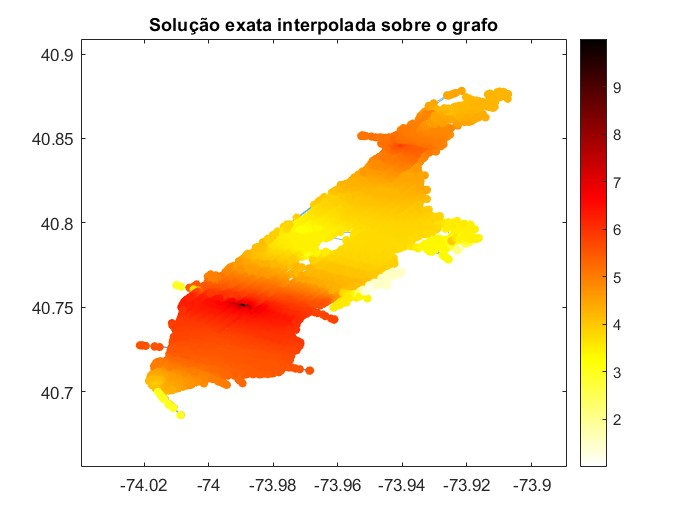
\includegraphics[width=\textwidth]{exactsolution.jpeg}
                \pause
                \caption{\scriptsize{Buscamos uma solução dessa forma.}}
            \end{column}
            
        \end{columns}
    \end{frame}

    \begin{frame}{Gauss-Jacobi}
        \pause
        \begin{columns}
            \begin{column}{0.5\textwidth}
               \begin{enumerate}
                   \item Convergiu com 1000 iterações e em 0.545334 segundo.
                    \pause
                    \item Este método foi o que mais divergiu do resultado exato, com uma norma $\ell^2$ da diferença de 3.768525e+02 e uma norma relativa de 8.318139e-01, o que justifica o mapa insatisfatório.
               \end{enumerate} 
            \end{column}
            \begin{column}{0.5\textwidth}
                \centering
                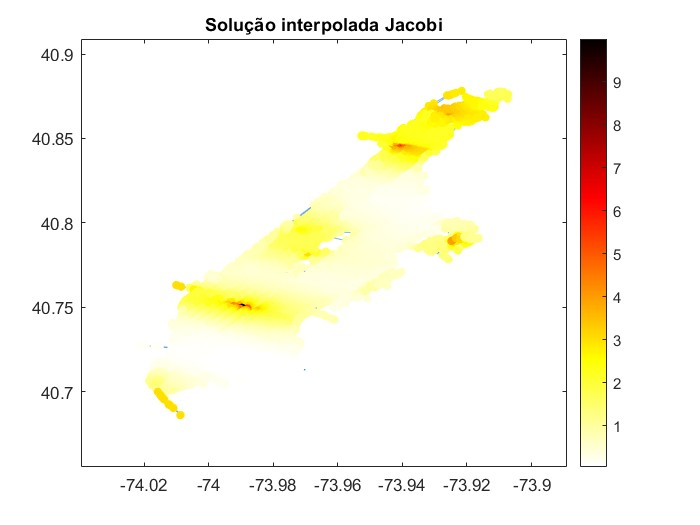
\includegraphics[width=\textwidth]{GJinterpol.jpeg}
            \end{column}
        \end{columns}
    \end{frame}

    \begin{frame}{Gauss-Seidel}
        \pause
        \begin{columns}
            \begin{column}{0.5\textwidth}
               \begin{enumerate}
                   \item Convergiu com 1000 iterações e em 0.368160 segundo.
                    \pause
                    \item Apesar de ter se aproximado mais da solução exata do que o método de Jacobi, com uma norma $\ell^2$ da diferença de 3.274648e+02 e uma norma relativa de 7.228020e-01, o método de Gauss-Seidel ainda resulta numa representação longe da ideal.
               \end{enumerate} 
            \end{column}
            \begin{column}{0.5\textwidth}
                \pause
                \centering
                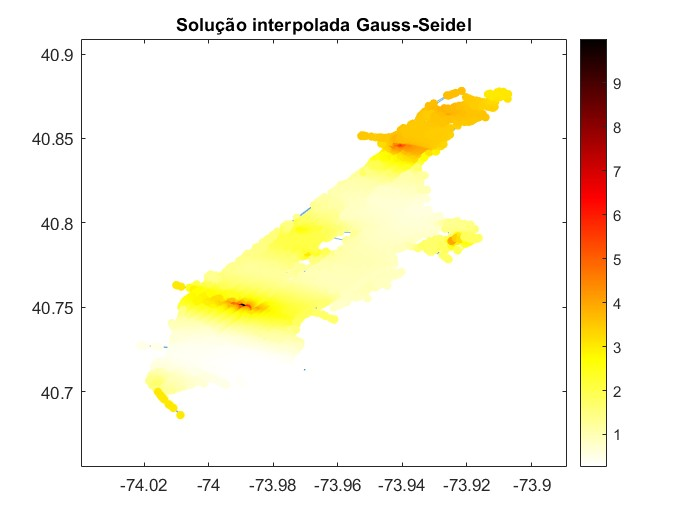
\includegraphics[width=\textwidth]{GSinterpol.jpeg}
            \end{column}
        \end{columns}
    \end{frame}

    \begin{frame}{Gradientes conjugados}
        \pause
        \begin{columns}
            \begin{column}{0.5\textwidth}            
                \begin{enumerate}
                    \item A convergência do método dos gradientes conjugados é garantida pelo fato de que a matriz  $L + P$ é simétrica definida positiva.
                    \pause
                    \item  O método CG convergiu com 1101 iterações e em 0.1703 segundo.
                    \pause
                    \item Convergiu eficientemente, com uma norma $\mathcal{\ell}^2$ da diferença em relação ao resultado exato de 3.172346e-05 e uma norma relativa de 7.002212e-08.
                    \pause
                \end{enumerate}
            \end{column}
            \begin{column}{0.5\textwidth}
                \centering
                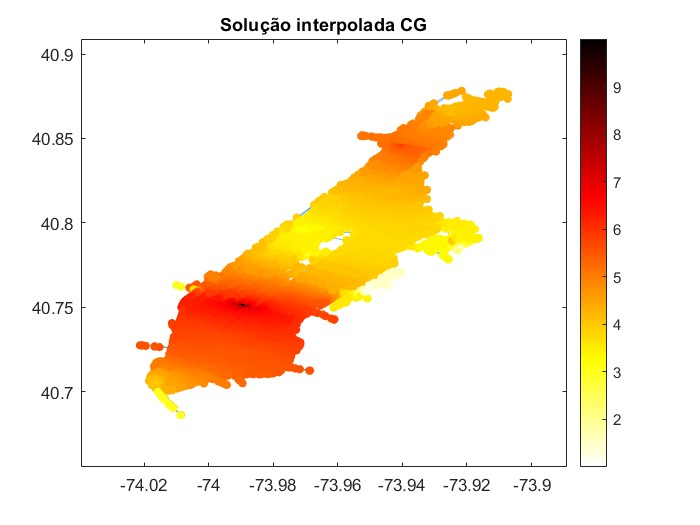
\includegraphics[width=\textwidth]{CGinterpol.jpeg}
            \end{column}
        \end{columns}
    \end{frame}

    \begin{frame}{Interpretando os resultados}

    \end{frame}
\end{document}
